\documentclass[../part_1.tex]{subfiles}

\begin{document}
    \subsubsection{DINO}
    % #TODO Не существет обоснования почему решение задачи млм способствует получению информации обо всем тексте
    \par Интуитивно кажется что решение задачи \acrshort{mlm} не способствует тому что модель будет понимать структуру кода или какие-либо отличительные черты. 
    % #TODO В последнее время большую популрность получил метод 
    \par В ходе исследования внимание было обращено внимание на метод обучения \acrshort{dino}\cite{caron2021emergingpropertiesselfsupervisedvision,oquab2024dinov2learningrobustvisual,darcet2024visiontransformersneedregisters} разработанный FacebookResearch. % #TODO Этот алгоримт представляет собой способ эффективного извлечения признаков, можно Он позволяет эффективно обучать модели на изображениях без разметки, извлекать универсальные визуальные представления. 
    \par Ключевая идея \acrshort{dino} — обучение c "самодистилляцией", тоесть % #TODO от модели требуется относить векторы представления чего то кчему то.
    \par Для обучения используется две модели -- учитель и ученик. Учитель генерирует эталонные представления изображения, тогда как ученик пытается предсказать выход учителя. % #TODO Во время обучения изменяются веса ученика, а веса учителя являются экспоненциальным затуханием весов ученика на протяжении всего обучения, что позволяет модели обучать себя на предоставленных даннхы.
    % #TODO В основе обучения состоит получение двух семантически разных кропов. Первая группа назваемая глобальными представлет собой участки изображения содержащи большую его часть. Вторая группа называемая локальными кропами содержит лишь небольшую часть изображенияч. В процессе обучения модели необходимо правильно сопоставить локальные участки с глобальными участками. При этом к каждому набору участков применяется множество аугментаций, такие как отражения, изменение баланса цвета, измененеие ярксти, изменение контраста. Так же модель учителя рассматривает только глобальные участки а модель ученика глобальные и локальные.
    \par В процессе обучения изображения разделяются на участки. Сначала из изображения выделяются два глобальных участка(изображение включающее 90\% исходного). Затем из изображения выделяются шесть локальных участков (изображения включающие около 15\% исходного). После этого к каждому набору участок применяются аугментации(например отражение, изменение цветов и так далее) и глобальные участи передаются в учителя, а локальные в ученика.
    \begin{figure}[h]
        \centering
        % #TODO Сабфигур
        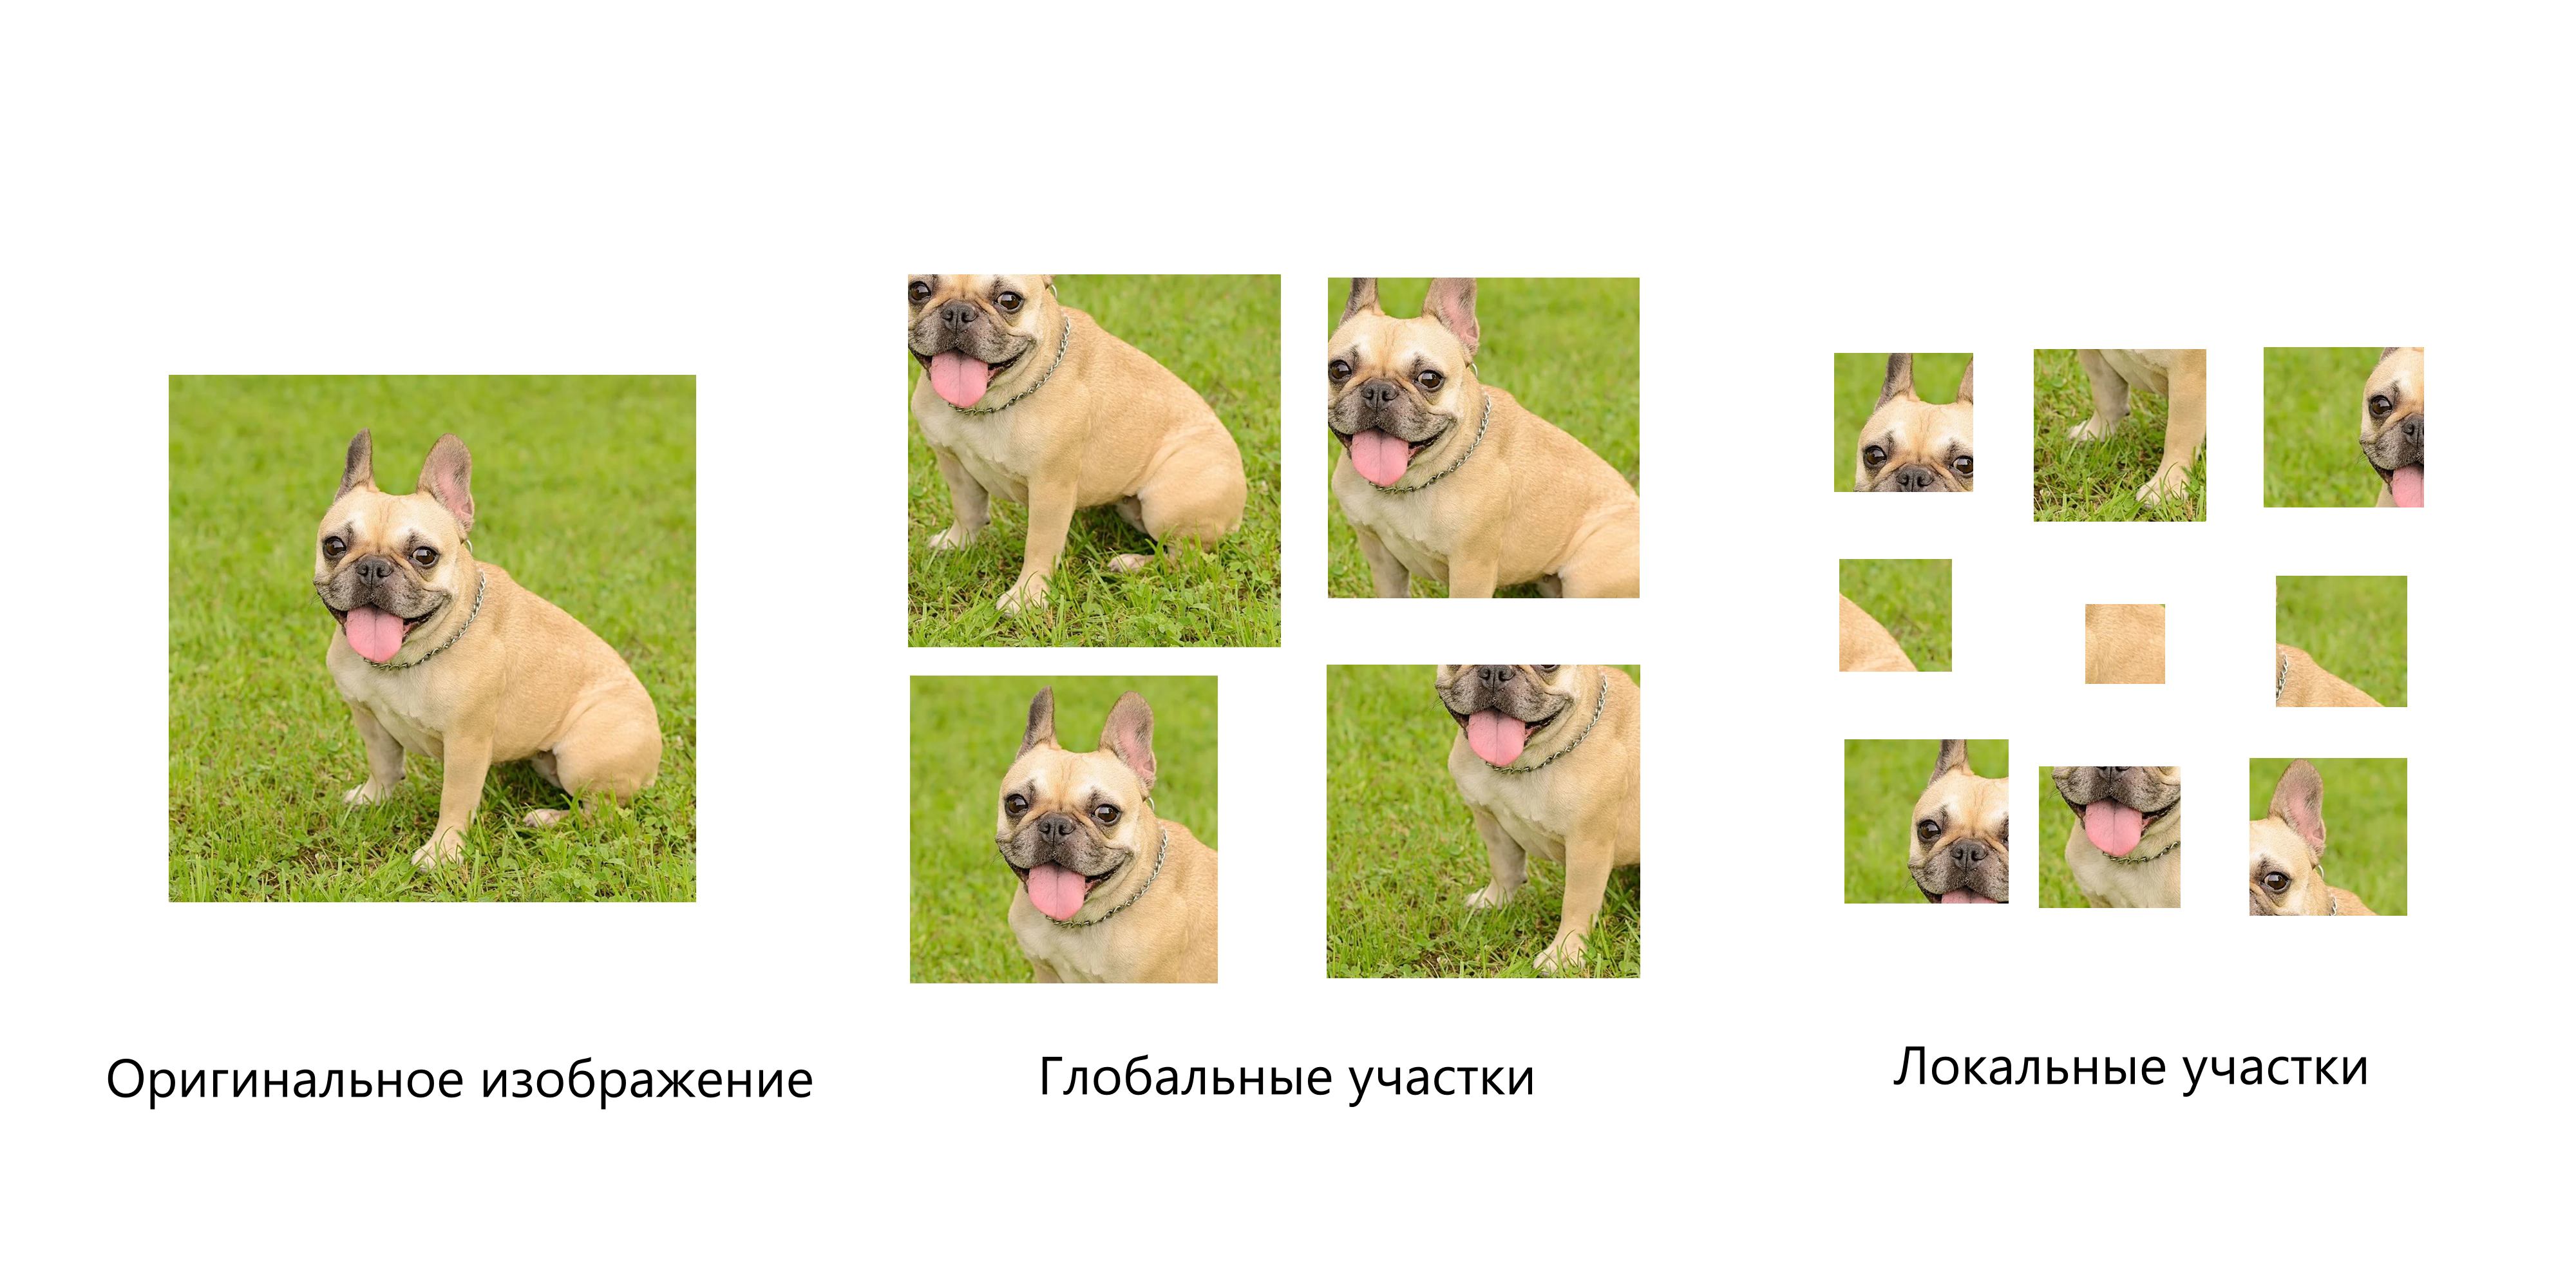
\includegraphics[width=0.8\textwidth]{multicrop_augment.png}
        \caption{Пример multicrop augmentation}
        \label{fig:multicrop_augment}
    \end{figure}
    % #TODO 
    \par Также в loss функции используется техника заострения(Sharpening), которая делает выходное вероятностное распределение более пиковым, уменьшая энтропию и подчеркивая наиболее вероятные классы. Это помогает избежать тривиальных решений, когда модель вырождается  и предсказывает равномерное распределение для всех входов. Sharpening выглядит как Softmax с параметром $\tau$
    \begin{equation}
        \label{sharpening}
        P(x)^{(i)} = \frac{exp\Big(\frac{g_\theta(x)^{(i)}}{\tau}\Big)}{\Sigma\limit^K_{k=1}exp\Big(\frac{g_\theta(x)^{(k)}}{\tau}\Big)}\,.
    \end{equation}
    % #TODO Представляет собой софтмакс с параметром тау
    
    \par В формуле \iqref{sharpening} показана функция sharpening для $i$ элемента модели $g$ с параметрами $\theta$. 
    % #TODO В алгоритме дино основной функцие потерь является кросс энтропия, длинное предложение.
    \begin{equation}
        \label{cross_entropy}
        Loss = -P_t(x) \log \P_s(x)\,.
    \end{equation}
    \par В формуле \iqref{cross_entropy} показана функция потерь для учителя и студента.
    \par В качестве Loss функции используется стандартная кросс этнтропия.
    % #TODO не ученик меняет а мы меняем
    \par В процессе обучения ученик изменяет свои веса таким образом чтобы уменьшить разницу предсказания с предсказанием учителя. Веса учителя постепенно изменяются обновбляясь как экспоненциальное скользящее среднее весов ученика.
    % #TODO Написать про все лоссы
\end{document}